%%%%%%%%%%%%%%%%%%%%%%%%%%%%% Define Article %%%%%%%%%%%%%%%%%%%%%%%%%%%%%%%%%%
% sets fontsize to 12
\documentclass[12]{article}
%%%%%%%%%%%%%%%%%%%%%%%%%%%%%%%%%%%%%%%%%%%%%%%%%%%%%%%%%%%%%%%%%%%%%%%%%%%%%%%

%%%%%%%%%%%%%%%%%%%%%%%%%%%%% Using Packages %%%%%%%%%%%%%%%%%%%%%%%%%%%%%%%%%%
\usepackage{geometry}
\usepackage{graphicx}
\usepackage{amssymb}
\usepackage{amsmath}
\usepackage{amsthm}
\usepackage{empheq}
\usepackage{mdframed}
\usepackage{booktabs}
\usepackage{lipsum}
\usepackage{graphicx}
\usepackage{color}
\usepackage{psfrag}
\usepackage{pgfplots}
\usepackage{bm}
\usepackage[english]{babel}
\usepackage[colorlinks=true, allcolors=blue]{hyperref}
\usepackage[onehalfspacing]{setspace}
\renewcommand{\familydefault}{\sfdefault}
\usepackage{nicematrix}

%%%%%%%%%%%%%%%%%%%%%%%%%%%%%%%%%%%%%%%%%%%%%%%%%%%%%%%%%%%%%%%%%%%%%%%%%%%%%%%

% extra settings here
% \newcommand\T{\rule{0pt}{2.6ex}}       % Top strut
% \newcommand\B{\rule[-1.2ex]{0pt}{0pt}} % Bottom strut

\newcommand\T{\rule{0pt}{3.5ex}}       % Top strut
\newcommand\I{\rule[-1.25ex]{0pt}{0pt}} % Inner strut
\newcommand\B{\rule[-2.0ex]{0pt}{0pt}} % Bottom strut
\PassOptionsToPackage{table}{xcolor}

%%%%%%%%%%%%%%%%%%%%%%%%%% Page Setting %%%%%%%%%%%%%%%%%%%%%%%%%%%%%%%%%%%%%%%
\geometry{a4paper,top=2.5cm,bottom=2.5cm,left=4cm,right=3cm,marginparwidth=1.75cm}

%%%%%%%%%%%%%%%%%%%%%%%%%% Define some useful colors %%%%%%%%%%%%%%%%%%%%%%%%%%
\definecolor{ocre}{RGB}{243,102,25}
\definecolor{mygray}{RGB}{243,243,244}
\definecolor{deepGreen}{RGB}{26,111,0}
\definecolor{shallowGreen}{RGB}{235,255,255}
\definecolor{deepBlue}{RGB}{61,124,222}
\definecolor{shallowBlue}{RGB}{235,249,255}
%%%%%%%%%%%%%%%%%%%%%%%%%%%%%%%%%%%%%%%%%%%%%%%%%%%%%%%%%%%%%%%%%%%%%%%%%%%%%%%

%%%%%%%%%%%%%%%%%%%%%%%%%% Define an orangebox command %%%%%%%%%%%%%%%%%%%%%%%%
\newcommand\orangebox[1]{\fcolorbox{ocre}{mygray}{\hspace{1em}#1\hspace{1em}}}
%%%%%%%%%%%%%%%%%%%%%%%%%%%%%%%%%%%%%%%%%%%%%%%%%%%%%%%%%%%%%%%%%%%%%%%%%%%%%%%

%%%%%%%%%%%%%%%%%%%%%%%%%%%% English Environments %%%%%%%%%%%%%%%%%%%%%%%%%%%%%
\newtheoremstyle{mytheoremstyle}{3pt}{3pt}{\normalfont}{0cm}{\rmfamily\bfseries}{}{1em}{{\color{black}\thmname{#1}~\thmnumber{#2}}\thmnote{\,--\,#3}}
\newtheoremstyle{myproblemstyle}{3pt}{3pt}{\normalfont}{0cm}{\rmfamily\bfseries}{}{1em}{{\color{black}\thmname{#1}~\thmnumber{#2}}\thmnote{\,--\,#3}}
\theoremstyle{mytheoremstyle}
\newmdtheoremenv[linewidth=1pt,backgroundcolor=shallowGreen,linecolor=deepGreen,leftmargin=0pt,innerleftmargin=20pt,innerrightmargin=20pt,]{theorem}{Theorem}[section]
\theoremstyle{mytheoremstyle}
\newmdtheoremenv[linewidth=1pt,backgroundcolor=shallowBlue,linecolor=deepBlue,leftmargin=0pt,innerleftmargin=20pt,innerrightmargin=20pt,]{definition}{Definition}[section]
\theoremstyle{myproblemstyle}
\newmdtheoremenv[linecolor=black,leftmargin=0pt,innerleftmargin=10pt,innerrightmargin=10pt,]{problem}{Problem}[section]
%%%%%%%%%%%%%%%%%%%%%%%%%%%%%%%%%%%%%%%%%%%%%%%%%%%%%%%%%%%%%%%%%%%%%%%%%%%%%%%

%%%%%%%%%%%%%%%%%%%%%%%%%%%%%%% Plotting Settings %%%%%%%%%%%%%%%%%%%%%%%%%%%%%
\usepgfplotslibrary{colorbrewer}
\pgfplotsset{width=8cm,compat=1.9}
%%%%%%%%%%%%%%%%%%%%%%%%%%%%%%%%%%%%%%%%%%%%%%%%%%%%%%%%%%%%%%%%%%%%%%%%%%%%%%%

%%%%%%%%%%%%%%%%%%%%%%%%%%%%%%% Title & Author %%%%%%%%%%%%%%%%%%%%%%%%%%%%%%%%
\title{Argument Component Identification im Stile von Stab und Gurevych}
\author{Hugo Meinhof, 815220}
%%%%%%%%%%%%%%%%%%%%%%%%%%%%%%%%%%%%%%%%%%%%%%%%%%%%%%%%%%%%%%%%%%%%%%%%%%%%%%%

\begin{document}
  \maketitle
  \begin{abstract}
  some abstract stuff goes here Stab und Gurevych\cite{stab-gurevych-2017-parsing}
  \end{abstract}
  \section{introduction\dotfill}
  \subsection{Previous Work: Stab and Gurevych 2017}
  In 2017, Stab and Gurevych\cite{stab-gurevych-2017-parsing} revisited their own work on argumentation mining from 2014. Dissatisfied with the existing corpora at the time, they decided to make their own, which they extended in 2017. On that corpus of persuasive essays, they annotated argument components and their argumentation structures. on these annotations, they trained models to built and tested a pipeline. 
  ``However, our identification model yields good accuracy and an $\alpha_U$ of 0.958 for identifying argument components. Therefore, it is unlikely that identification errors will significantly influence the outcome of the downstream models when applied to persuasive essays.'' meaning that they didnt evaluate the entire pipeline, as they expect to get the same results as the models, running on gold data. This is a questionable practice, expecially considering that they're focussing on the accuracy, and not f1 here. \textcolor{red}{cant find the accuracy referenced here}
  ``However, as demonstrated by Levy et al. (2014) and Goudas et al.
(2014), the identification of argument components is more complex in other text genres
than it is in persuasive essays. Another potential issue of the pipeline architecture is that
wrongly classified major claims will decrease the accuracy of the model because they
are not integrated in the joint modeling approach. For this reason, it is worthwhile to
experiment in future work with structured machine learning methods that incorporate
several tasks in one model (Moens 2013).'' I have trained such model, full\_labels, which sadly doesnt reach the f1 of the SuG ILP model yet.
  \subsection{Goal of my work}
  For this paper I have attempted to surpass the models for argument component identification and classification, as shown in Figure~\ref{fig:model_tree}. In general, the identification regards the question of where an argument component, like MajorClaim, will be located, without knowing what type it will be. Then, the classification task is the labeling of what kind of argument component we are dealing with. Stab and Gurevych trained models for each task, and my goal was to surpass them.  \textcolor{red}{ELABORATE AND REFERENCE FIGURE -- eplain what a span is} 
  \begin{figure}[!h]
    \centering
    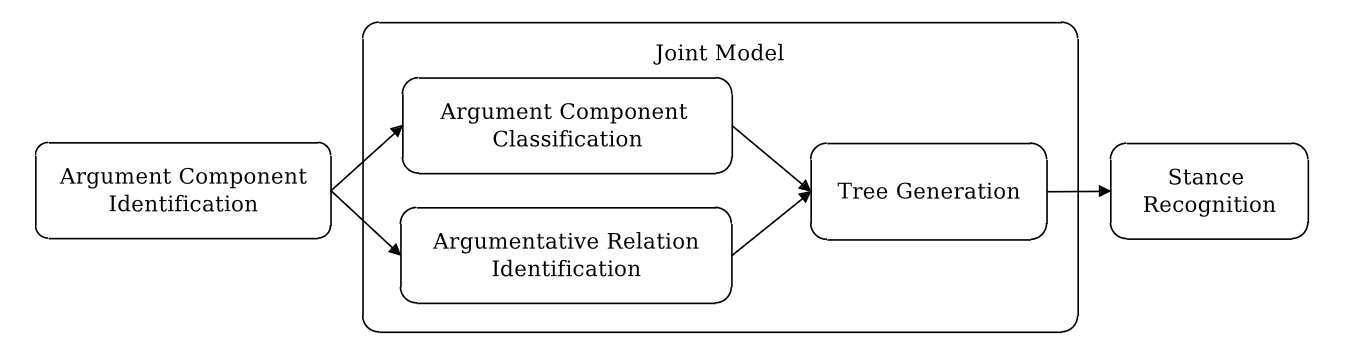
\includegraphics[width=1\linewidth]{../s-g_model_tree.png}
    \caption{Architecture of the argumentation structure parser.}
    \label{fig:model_tree}
  \end{figure}
  \subsection{my previous work}
  test
  \section{Finding Argumentation Components}
  I have trained and compared multiple models and methods for both identifying and classifying argumentation components. From that process, five different models emerged, in various stages of simplification and mutual support. All of them are finetuned versions of longformer\cite{beltagy2020longformer}, the long document transformer.
  \subsection{full labels}
  Just like Stab and Gurevych recommended in 2017, I tried to train a model that combined the tasks of argument component identification and classification. For that I used the labels ``B-MajorClaim'', ``I-MajorClaim'', ``B-Claim'', ``I-Claim'',``B-Premise'', ``I-Premise'', and ``O''. The first Part of each label carries information for the argument component identification, whilst the second part does so for the classification. Full labels performs worse than Stab and Gurevychs ILP-balanced model\cite{stab-gurevych-2017-parsing}. However this is not an apples to apples comparison, as there is no 5-fold cross-validated evaluation data available for the pipeline, with the ILP model, meaning that it may perform worse than the full labels model. 
  \subsection{spans}
  Once again, just like Stab and Gurevych in 2017, i came to realise that splitting up the argument component identification and classification could yield overall improvements. The spans model takes care of the first part of the pipeline, the identification. It uses the labels ``B'', ``I'', and ``O''. Reducing the number of labels from seven to three, and limiting the task to identifying the spans, greatly improved the models performance, compared to full labels.
  \subsection{simple}
  With the performance increase of the spans model in mind, I created the simple model. It uses the labels ``MajorClaim'', ``Claim'', ``Premise'', ``X\_placeholder\_X'', and ``O''.The X\_placeholder\_X label however is never annotated in the entire dataset, and hence never used. I discuss it in the section \ref{problems}.
 The idea of this model is the exact same as with the simple model, except this time its for the classification task instead of identification. The lack of information regarding where spans are, would be made up for in the post processing. There, for each span that has been found by the spans model, the pipeline would check what labels were annotated. The most commonly annotated label within the span would then be applied to the entire span.  
  \begin{verbatim}
``we'', ``should'', ``attach'', ``more'', ``importance'', ``to'', ``cooperation''
``O'', ``Claim'', ``Claim'', ``Premise'', ``Premise'', ``Claim'', ``Claim''
  \end{verbatim}
  This synthetic example shows a span without its context. Within it, Claim is the most commonly annotated label, and so the post processing would consider the entire span to be of the type ``Claim''.
  \subsection{sep tok full labels}
  This model takes advantage of another way in which the spans model can support a model that follows. Not only can the information on where spans are be used during post processing, but also before the inference or training. The preprocessing for this model places class and separator tokens in the text data, in order to signal where spans are. During pretraining, separator tokens ``which is used when building a sequence from multiple sequences, e.g. two sequences for sequence classification or for a text and a question for question answering. It is also used as the last token of a sequence built with special tokens.'' ``which is used when doing sequence classification (classification of the whole sequence instead of per-token classification). It is the first token of the sequence when built with special tokens.''
  \subsection{pipeline}
  \subsection{problems} \label{problems}
  - B and I labels are cool and all, but what use are they, when a span of labels begins with I, or when a random word is dropped from a span
  - i get cuda errors when running NER at an even number of labels. hence i am using X\_placeholder\_X.
  \section{trainingsdaten\dotfill}
  The foundation of the training data for this project consists of 402 student essays annotated by Stab and Gurevych. For each essay, the dataset includes information on where the core assertion of the text, otherwise known as the MajorClaim, supporting assertments, or the Claims, and the premises, that back up the thesis with statistics and other evidence, are located. 
The texts used were sourced from essayforum.com and selected randomly. No further information is known about the authors, but it is conceivable that English may not be their first language and they are likely learning it in an educational context.
Stab and Gurevych subsequently annotated the essays with tokens and recorded the locations of spans.

  quelle: https://aclanthology.org/J17-3005.pdf

  Claim: semantische klasse, die eine behauptung aufstellt; stützt majorclaim 
  MajorClaim: kernbehauptung(en) des textes 
  prämissen: unterstützung/ untermauerung der Claims (zb statistiken) 

  über baselines schreiben!

  ``For finding the best-performing models, we conduct model selection on our training data using 5-fold cross-validation''


  die essays wurden tokenisiert und gespeichert wo sich spannen befinden, welche rolle sie haben, und welche tokens dazugehören. diese daten werden von renes script erstellt was war das. damit modeelle damit lernen können, muss ein dataset erstellt werden, welches die daten aufbereitet und dem modell verständlich sortiert. dies ist die größte aufgabe beim training. da alle traininerten modelle auf dem selben datensatz basieren, gibt es für alle zusammen ein gemeinsames dataset. viele extraktions, aufbereitungs, und matching schritte bleiben für alle modelle gleich. unterschiede gibt es im grunde nur im letzten aufbereitungsschritt. das wird von den verschiedenen configs des datasets gehandhabt. es gibt für jedes modell eine eigene config, die den selben namen trägt, wie das modell. da sich die modelle nur darin unterscheiden wie die trainingsdaten aufbereitet sind, bedeutet das auch, dass ein trainingsscript für alle modelle verwendet werden kann, in dem nur die config angepasst werden muss. ich habe zudem darauf geachtet, dass die configs die selben namen tragen wie die modelle, damit alles reibungslos abläuft bessere erklärung des trainings scripts. das war jedoch nicht schon immer so. angefangen habe ich mit je einem trainings script pro modell. das ist zwar auf der einen seite nicht so anpassbar wie ein sript für alle, welches über command line arguments angepasst werden kann, hat jedoch auf der anderen seite den klaren vorteil, dass so ein einzelnes modell erstmal trainiert und ausgetestet werden kann, ohne dabei andere im hinterkopf behalten zu müssen. 

The corpus consists of 402 essays, downloaded, and randomly selected, from essayforum.com. 
  \section{evaluation\dotfill}
  \begin{table}[!h]
    \centering
    \begin{NiceTabular}{c||c|c|c|c|c} 
      \CodeBefore
        \rowcolors{2}{gray!25}{white}
      \Body
      \textbf{Makro-f1} & \textbf{full labels} & \textbf{spans} & \textbf{simple} & \textbf{sep tok full labels} & \textbf{sep tok} \\ 
      \hline
      \hline
      4 & 0.579 & 0.898 & 0.769 & 0.749 & 0.843\T\\
      5 & 0.631 & 0.905 & 0.782 & 0.801 & 0.849\\
      6 & 0.716 & 0.908 & 0.790 & 0.816 & 0.858\\
      7 & 0.740 & 0.910 & 0.796 & 0.824 & 0.864\\
      8 & 0.752 & 0.911 & 0.800 & 0.832 & 0.864\\
      9 & 0.757 & 0.912 & 0.801 & 0.837 & 0.865\\
      10 & 0.759 & 0.912 & 0.801 & 0.838 & 0.867\\
      11 & 0.761 & 0.912 & 0.803 & 0.833 & 0.866\\
      12 & 0.763 & 0.914 & 0.803 & 0.837 & 0.865\\
      13 & 0.763 & 0.913 & 0.802 & 0.844 & 0.867\\
      14 & 0.767 & 0.915 & 0.801 & 0.840 & 0.867\\
      15 & 0.766 & 0.914 & 0.801 & 0.841 & 0.868\\
      16 & 0.766 & 0.915 & 0.803 & 0.846 & 0.870\\
    \end{NiceTabular}
    \vfill
    \caption{5-fold cross-validation of the macro-f1}
    \label{tab:epoch_f1}
  \end{table}


  \begin{table}[!h]
    \centering
    \begin{NiceTabular}{c|c}[colortbl-like]
      \large\textbf{Argument Component Identification} &  \large\textbf{Makro-f1}\\ 
      \hline
      \hline
      \textbf{Stab und Gurevytch}& \T \I \\
      \rowcolor{gray!25}
      Human upper bound & 0.886\\
      Baseline majority & 0.259\\
      \rowcolor{gray!25}
      Baseline heuristic & 0.628\\
      \textbf{CRF all features} & \textbf{0.849}\B\\
      \hline
      \textbf{Meinhof} & \T \I \\
      \rowcolor{gray!25}
      \textbf{spans} & \textbf{0.912}\\ 
    \end{NiceTabular}
    \caption{Argument Component Identification (5-fold cross-validation as in Table C.1 of \cite{stab-gurevych-2017-parsing})}
    \label{tab:ident_f1}
  \end{table}

  \begin{table}[!h]
    \centering
    \begin{NiceTabular}{c|c}[colortbl-like]
      \large\textbf{Argument Component Classification} &  \large\textbf{Makro-f1}\\
      \hline
      \hline
      \textbf{Stab und Gurevych} & \T \I \\
      \rowcolor{gray!25}
      Baseline majority & 0.257\\
      Baseline heuristic & 0.724\\
      \rowcolor{gray!25}
      \textbf{SVM all features} & \textbf{0.773}\\
      \textbf{ILP-balanced} & \textbf{0.823}\\
      \rowcolor{gray!25}
      \textit{ILP and CRF} & no-eval \B \\
      \hline
      \textbf{Meinhof} & \T \I \\
      \rowcolor{gray!25}
      full\_labels & 0.759\\
      simple & 0.801\\
      \rowcolor{gray!25}
      sep\_tok\_full\_labels & 0.838\\
      \textbf{sep\_tok} & \textbf{0.867}\\
      \rowcolor{gray!25}
      \textit{full\_pipe} & \textit{TO-DO}\\

    \end{NiceTabular}
    \caption{Argument Component Classification (5-fold cross-validation as in Table C.2 of \cite{stab-gurevych-2017-parsing})}
    \label{tab:class_f1}
  \end{table}

  \section{training\dotfill}
  \newpage
  \bibliographystyle{alpha}
  \bibliography{../notes}
\end{document}
